% Options for packages loaded elsewhere
\PassOptionsToPackage{unicode}{hyperref}
\PassOptionsToPackage{hyphens}{url}
%
\documentclass[
  letterpaper,
  ignorenonframetext,
  aspectratio=43,
  handout,
  12pt]{beamer}
\usepackage{pgfpages}
\setbeamertemplate{caption}[numbered]
\setbeamertemplate{caption label separator}{: }
\setbeamercolor{caption name}{fg=normal text.fg}
\beamertemplatenavigationsymbolsempty
% Prevent slide breaks in the middle of a paragraph
\widowpenalties 1 10000
\raggedbottom
\setbeamertemplate{part page}{
  \centering
  \begin{beamercolorbox}[sep=16pt,center]{part title}
    \usebeamerfont{part title}\insertpart\par
  \end{beamercolorbox}
}
\setbeamertemplate{section page}{
  \centering
  \begin{beamercolorbox}[sep=12pt,center]{part title}
    \usebeamerfont{section title}\insertsection\par
  \end{beamercolorbox}
}
\setbeamertemplate{subsection page}{
  \centering
  \begin{beamercolorbox}[sep=8pt,center]{part title}
    \usebeamerfont{subsection title}\insertsubsection\par
  \end{beamercolorbox}
}
\AtBeginPart{
  \frame{\partpage}
}
\AtBeginSection{
  \ifbibliography
  \else
    \frame{\sectionpage}
  \fi
}
\AtBeginSubsection{
  \frame{\subsectionpage}
}
\usepackage{amsmath,amssymb}
\usepackage{lmodern}
\usepackage{iftex}
\ifPDFTeX
  \usepackage[T1]{fontenc}
  \usepackage[utf8]{inputenc}
  \usepackage{textcomp} % provide euro and other symbols
\else % if luatex or xetex
  \usepackage{unicode-math}
  \defaultfontfeatures{Scale=MatchLowercase}
  \defaultfontfeatures[\rmfamily]{Ligatures=TeX,Scale=1}
\fi
\usetheme[]{metropolis}
% Use upquote if available, for straight quotes in verbatim environments
\IfFileExists{upquote.sty}{\usepackage{upquote}}{}
\IfFileExists{microtype.sty}{% use microtype if available
  \usepackage[]{microtype}
  \UseMicrotypeSet[protrusion]{basicmath} % disable protrusion for tt fonts
}{}
\makeatletter
\@ifundefined{KOMAClassName}{% if non-KOMA class
  \IfFileExists{parskip.sty}{%
    \usepackage{parskip}
  }{% else
    \setlength{\parindent}{0pt}
    \setlength{\parskip}{6pt plus 2pt minus 1pt}}
}{% if KOMA class
  \KOMAoptions{parskip=half}}
\makeatother
\usepackage{xcolor}
\IfFileExists{xurl.sty}{\usepackage{xurl}}{} % add URL line breaks if available
\IfFileExists{bookmark.sty}{\usepackage{bookmark}}{\usepackage{hyperref}}
\hypersetup{
  hidelinks,
  pdfcreator={LaTeX via pandoc}}
\urlstyle{same} % disable monospaced font for URLs
\newif\ifbibliography
\usepackage{graphicx}
\makeatletter
\def\maxwidth{\ifdim\Gin@nat@width>\linewidth\linewidth\else\Gin@nat@width\fi}
\def\maxheight{\ifdim\Gin@nat@height>\textheight\textheight\else\Gin@nat@height\fi}
\makeatother
% Scale images if necessary, so that they will not overflow the page
% margins by default, and it is still possible to overwrite the defaults
% using explicit options in \includegraphics[width, height, ...]{}
\setkeys{Gin}{width=\maxwidth,height=\maxheight,keepaspectratio}
% Set default figure placement to htbp
\makeatletter
\def\fps@figure{htbp}
\makeatother
% Make links footnotes instead of hotlinks:
\DeclareRobustCommand{\href}[2]{#2\footnote{\url{#1}}}
\setlength{\emergencystretch}{3em} % prevent overfull lines
\providecommand{\tightlist}{%
  \setlength{\itemsep}{0pt}\setlength{\parskip}{0pt}}
\setcounter{secnumdepth}{-\maxdimen} % remove section numbering
\usepackage{pgfpages}
\pgfpagesuselayout{2 on 1}
\providecommand{\tightlist}{%
\setlength{\itemsep}{0pt}\setlength{\parskip}{0pt}}
\makeatletter
\makeatother
\let\Oldincludegraphics\includegraphics
\renewcommand{\includegraphics}[2][]{\Oldincludegraphics[width=\textwidth,height=0.7\textheight,keepaspectratio]{#2}}
\ifLuaTeX
  \usepackage{selnolig}  % disable illegal ligatures
\fi

\author{}
\date{}

\begin{document}

\hypertarget{ae731}{%
\section{AE731}\label{ae731}}

\begin{frame}{Theory of Elasticity}
\protect\hypertarget{theory-of-elasticity}{}
Dr.~Nicholas Smith

Wichita State University, Department of Aerospace Engineering 23
September, 2021
\end{frame}

\begin{frame}{upcoming schedule}
\protect\hypertarget{upcoming-schedule}{}
\begin{itemize}
\tightlist
\item
  Sep 23 - Material Characterization
\item
  Sep 24 - Homework 3 Due
\item
  Sep 28 - Thermoelasticity
\item
  Sep 30 - Boundary Conditions
\item
  Oct 1 - Homework 3 Self-grade Due, Homework 4 Due
\end{itemize}
\end{frame}

\begin{frame}{outline}
\protect\hypertarget{outline}{}
\begin{itemize}
\tightlist
\item
  review
\item
  material characterization
\item
  hooke's law
\item
  matrix relationship
\item
  physical meaning
\end{itemize}
\end{frame}

\hypertarget{review}{%
\section{review}\label{review}}

\begin{frame}{example}
\protect\hypertarget{example}{}
\begin{columns}[T]
\begin{column}{0.5\textwidth}
\begin{itemize}
\tightlist
\item
  Suppose a hanging cylinder has a density given by \(\rho = r^2\)
\item
  Self-weight is the only force acting on this problem
\end{itemize}
\end{column}

\begin{column}{0.5\textwidth}
\begin{figure}
\centering
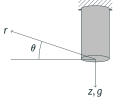
\includegraphics{../images/11-example.svg}
\caption{drawing of the problem described}
\end{figure}
\end{column}
\end{columns}
\end{frame}

\begin{frame}{example}
\protect\hypertarget{example-1}{}
\begin{itemize}
\item
  We know that there is no traction along the outer surfaces, and we can
  also assume that \(\sigma_{ij} = \sigma_{ij}(z)\), since the only
  force is acting in the z direction
\item
  Using Cauchy's stress theorem we can find
\end{itemize}

\[\begin{aligned}
    t_j &= \sigma_{ij} n_i = 0\\
    &= \langle \sigma_{rr}n_r + \sigma_{r\theta} n_\theta + \sigma_{rz} n_z, \sigma_{\theta r}n_r + \sigma_{\theta \theta} n_\theta + \sigma_{\theta z} n_z, \sigma_{zr}n_r + \sigma_{z\theta} n_\theta + \sigma_{zz} n_z\rangle \\
    &= \langle \sigma_{rr}, \sigma_{\theta r}, \sigma_{z r} \rangle = 0 \qquad \text{at } r=a
\end{aligned}\]
\end{frame}

\begin{frame}{example}
\protect\hypertarget{example-2}{}
\begin{itemize}
\tightlist
\item
  And on the bottom face
\item
  \(\sigma_{rz} = \sigma_{\theta z} = \sigma_{zz} = 0\)
\end{itemize}
\end{frame}

\begin{frame}{example}
\protect\hypertarget{example-3}{}
\begin{itemize}
\tightlist
\item
  To find the stress in the \emph{z} direction, we use the third
  equilibrium equation
\end{itemize}

\[\frac{\partial \tau_{r z}}{\partial r} + \frac{1}{r} \frac{\partial \tau_{\theta z}}{\partial \theta} + \frac{\partial \sigma_z}{\partial z} + \frac{1}{r}\tau_{rz} + F_z = 0\]

\begin{itemize}
\tightlist
\item
  We can substitute known values to find that
\end{itemize}

\[\frac{\partial \sigma_z}{\partial z} + r^2 g = 0\]
\end{frame}

\begin{frame}{example}
\protect\hypertarget{example-4}{}
\begin{columns}[T]
\begin{column}{0.5\textwidth}
\begin{itemize}
\tightlist
\item
  Since we desire to find the stress at any point, we introduce a
  variable to indicate the coordinate of our free body diagram cut
\end{itemize}
\end{column}

\begin{column}{0.5\textwidth}
\begin{figure}
\centering
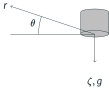
\includegraphics{../images/11-example-2.svg}
\caption{section cut of hanging cylinder}
\end{figure}
\end{column}
\end{columns}
\end{frame}

\begin{frame}{example}
\protect\hypertarget{example-5}{}
\begin{itemize}
\tightlist
\item
  We integrate over this free body to find
\end{itemize}

\[\begin{aligned}
    \sigma_z &=  -\int_\zeta^{-L} r^2 g dz\\
    &= r^2 g (L-z)
\end{aligned}\]

\begin{itemize}
\tightlist
\item
  In this case, the stress is a function of radial distance (just like
  the body force was)
\end{itemize}
\end{frame}

\begin{frame}{example}
\protect\hypertarget{example-6}{}
\begin{itemize}
\tightlist
\item
  We can find the average stress at some location, \emph{z}
\end{itemize}

\[\bar{\sigma}_z = \frac{1}{A} \int \sigma_z dA\]

\begin{itemize}
\tightlist
\item
  In this case this integral becomes
\end{itemize}

\[\bar{\sigma}_z = \frac{1}{A} \int_0^R \int_0^{2\pi} r^2 g (L-z) r dr d\theta\]
\[\bar{\sigma}_z = \frac{1}{\pi R^2} \int_0^R 2 \pi r^3 g (L-z) dr\]
\[\begin{aligned}
    \bar{\sigma}_z &= \frac{2 \pi }{4 \pi R^2} R^4 g (L-z)\\
    &= \frac{R^2}{2} g (L-z)
\end{aligned}\]
\end{frame}

\hypertarget{material-characterization}{%
\section{material characterization}\label{material-characterization}}

\begin{frame}{material characterization}
\protect\hypertarget{material-characterization-1}{}
\begin{itemize}
\tightlist
\item
  We have now formally defined stress and strain tensors, it is
  desirable to relate these two tensors to one another
\item
  In this course we make the following assumptions about material
  behavior:

  \begin{itemize}
  \tightlist
  \item
    Small strains
  \item
    Linear elastic
  \item
    Rate-independent
  \item
    Homogeneous
  \end{itemize}
\end{itemize}
\end{frame}

\begin{frame}{tensile test}
\protect\hypertarget{tensile-test}{}
\begin{figure}
\centering
\includegraphics{../images/tensile_test.PNG}
\caption{tensile test}
\end{figure}
\end{frame}

\begin{frame}{shear tests}
\protect\hypertarget{shear-tests}{}
\includegraphics{../images/shear2.jpg}
\end{frame}

\begin{frame}{shear tests}
\protect\hypertarget{shear-tests-1}{}
\begin{figure}
\centering
\includegraphics{../images/shear4.jpg}
\caption{another shear test}
\end{figure}
\end{frame}

\hypertarget{hookes-law}{%
\section{hooke's law}\label{hookes-law}}

\begin{frame}{hooke's law}
\protect\hypertarget{hookes-law-1}{}
\begin{itemize}
\tightlist
\item
  In its most general form, Hooke's Law relates the stress and strain
  tensors by the Cauchy stiffness tensor
\end{itemize}

\[\sigma_{ij} = C_{ijkl} \epsilon_{kl}\]

\begin{itemize}
\tightlist
\item
  We could, equivalently write this equation in terms of the compliance
\end{itemize}

\[\epsilon_{ij} = S_{ijkl}\sigma_{kl}\]
\end{frame}

\begin{frame}{hooke's law}
\protect\hypertarget{hookes-law-2}{}
\begin{itemize}
\tightlist
\item
  There are 81 terms in \(C_{ijkl}\) (3x3x3x3)
\item
  Many of these are redundant, so a contracted notation is sometimes
  convenient.
\item
  Symmetry of the stress tensor and strain tensors requires symmetries
  in \(C_{ijkl}\)
\end{itemize}

\[\begin{aligned}
    \sigma_{ij} &= C_{ijkl}\epsilon_{kl}\\
    &= \sigma_{ji}\\
    &= C_{jikl} \epsilon_{kl}\\
\end{aligned}\]

\begin{itemize}
\tightlist
\item
  \(C_{ijkl} = C_{jikl}\)
\item
  \(C_{ijkl} = C_{ijlk}\)
\end{itemize}
\end{frame}

\begin{frame}{hooke's law}
\protect\hypertarget{hookes-law-3}{}
\begin{itemize}
\tightlist
\item
  Strain energy concepts further require that \(C_{ijkl} = C_{klij}\)
\item
  This reduces the number of unique, unknown constants to 21
\item
  In general, if we cannot make any assumptions about material symmetry,
  there are 21 parameters that we need to find to determine the linear
  behavior of a material.
\end{itemize}
\end{frame}

\hypertarget{matrix-relationship}{%
\section{matrix relationship}\label{matrix-relationship}}

\begin{frame}{matrix form}
\protect\hypertarget{matrix-form}{}
\begin{itemize}
\tightlist
\item
  For this reason (as well as convenience in writing), many will often
  form a matrix equation, with \(\sigma\) and \(\epsilon\) acting as
  vectors.
\end{itemize}
\end{frame}

\begin{frame}{matrix form}
\protect\hypertarget{matrix-form-1}{}
\[\begin{Bmatrix}
    \sigma_1 \ \sigma_2 \ \sigma_3 \ \sigma_4 \ \sigma_5 \ \sigma_6
    \end{Bmatrix} = \begin{bmatrix}
    C_{11} & C_{12} & C_{13} & C_{14} & C_{15} & C_{16}\\
    C_{21} & C_{22} & C_{23} & C_{24} & C_{25} & C_{26}\\
    C_{31} & C_{32} & C_{33} & C_{34} & C_{35} & C_{36}\\
    C_{41} & C_{42} & C_{43} & C_{44} & C_{45} & C_{46}\\
    C_{51} & C_{52} & C_{53} & C_{54} & C_{55} & C_{56}\\
    C_{61} & C_{62} & C_{63} & C_{64} & C_{65} & C_{66}\\
    \end{bmatrix} \begin{Bmatrix}
    \epsilon_1 \ \epsilon_2 \ \epsilon_3 \ 2\epsilon_4 \ 2\epsilon_5 \ 2\epsilon_6
\end{Bmatrix}\]

\begin{itemize}
\tightlist
\item
  In this form, the usual tensor transformation equations cannot be
  used. Also, be careful as \(\sigma_4\), \(\sigma_5\) and \(\sigma_6\)
  do not always represent the same terms (depends on
  textbook/community), also sometimes the engineering form of shear
  (\(\gamma_{12} = 2\epsilon_{12}\)) is used.
\end{itemize}
\end{frame}

\begin{frame}{matrix form}
\protect\hypertarget{matrix-form-2}{}
\begin{itemize}
\tightlist
\item
  If we consider the \(\sigma_{11}\) term, we find that
\end{itemize}

\[\begin{aligned}
    \sigma_{11} &= C_{11kl} \epsilon_{kl}\\
    &= C_{1111} \epsilon_{11} + C_{1112} \epsilon_{12} + C_{1113} \epsilon_{13} + \\
    &C_{1121} \epsilon_{21} + C_{1122} \epsilon_{22} + C_{1123} \epsilon_{23} + \\
    &C_{1131} \epsilon_{31} + C_{1132} \epsilon_{32} + C_{1133} \epsilon_{33} \\
\end{aligned}\]

\begin{itemize}
\tightlist
\item
  If we simplify this, we find
\end{itemize}

`\$\sigma\emph{\{11\} = C}\{1111\}\epsilon\emph{\{11\} +
2C}\{1112\}\epsilon\emph{\{12\} + 2C}\{1113\}\epsilon\emph{\{13\} +
C}\{1122\}\epsilon\emph{\{22\} + 2C}\{1123\}\epsilon\emph{\{23\} +
C}\{1133\}\epsilon\_\{33\}\textbackslash{]}
\end{frame}

\begin{frame}{matrix form}
\protect\hypertarget{matrix-form-3}{}
\begin{itemize}
\tightlist
\item
  In matrix form, we write the normal terms first, and we include the
  factor of 2 in the strain vector, giving
\end{itemize}

\[\sigma_1 = C_{11} \epsilon_1 + C_{12} \epsilon_2 + C_{13} \epsilon_3 + C_{14} \epsilon_4 + C_{15} \epsilon_5 + C_{16} \epsilon_6 \]
\end{frame}

\hypertarget{physical-meaning}{%
\section{physical meaning}\label{physical-meaning}}

\begin{frame}{physical meaning}
\protect\hypertarget{physical-meaning-1}{}
\begin{itemize}
\tightlist
\item
  We will discuss symmetries in greater detail in a later lecture
\item
  An isotropic material reduces the unknown material constants to two
\end{itemize}

\[\epsilon_{ij} = \frac{1+\nu}{E}\sigma_{ij} - \frac{\nu}{E}\sigma_{kk} \delta_{ij}\]
\end{frame}

\begin{frame}{simple tension}
\protect\hypertarget{simple-tension}{}
\includegraphics{../images/uniaxial_tension.jpg}
\end{frame}

\begin{frame}{strain measurement}
\protect\hypertarget{strain-measurement}{}
\begin{itemize}
\tightlist
\item
  How do we measure strain?

  \begin{itemize}
  \tightlist
  \item
    grip displacement
  \item
    extensometers
  \item
    strain gages
  \item
    digital image correlation
  \end{itemize}
\end{itemize}
\end{frame}

\begin{frame}{extensometers}
\protect\hypertarget{extensometers}{}
\begin{itemize}
\tightlist
\item
  Reusable, quick to use, apply, and interpret
\item
  May slip, only gives one direction, can initiate failure site
\end{itemize}

\begin{figure}
\centering
\includegraphics{../images/extensometer.jpg}
\caption{image of extensometers}
\end{figure}
\end{frame}

\begin{frame}{strain gages}
\protect\hypertarget{strain-gages}{}
\begin{itemize}
\tightlist
\item
  Can be applied in any direction, very accurate
\item
  Must be perfectly adhered, subject to user-error in attaching, can
  require complicated electronics to read results
\end{itemize}

\includegraphics{../images/strain-gauge-on-specimen-.jpeg}
\end{frame}

\begin{frame}{digital image correlation}
\protect\hypertarget{digital-image-correlation}{}
\begin{columns}[T]
\begin{column}{0.5\textwidth}
\begin{itemize}
\tightlist
\item
  Gives full-field strain tensor
\item
  Requires expensive equipment, software
\item
  Cannot compute values near the edges
\end{itemize}
\end{column}

\begin{column}{0.5\textwidth}
\begin{figure}
\centering
\includegraphics{../images/dic.jpg}
\caption{image showing digital image correlation}
\end{figure}
\end{column}
\end{columns}
\end{frame}

\begin{frame}{simple tension}
\protect\hypertarget{simple-tension-1}{}
\begin{itemize}
\tightlist
\item
  If we consider a simple tension test, if done correctly the applied
  stress will be
\end{itemize}

\[\sigma_{ij} = \begin{bmatrix}
    \sigma & 0 & 0 \\
    0 & 0 & 0\\
    0 & 0 & 0
\end{bmatrix}\]

\begin{itemize}
\tightlist
\item
  What will the strain be?
\end{itemize}
\end{frame}

\begin{frame}{simple tension}
\protect\hypertarget{simple-tension-2}{}
\begin{itemize}
\tightlist
\item
  Recall Hooke's law for isotropic material
\end{itemize}

\[\epsilon_{ij} = \frac{1+\nu}{E}\sigma_{ij} - \frac{\nu}{E}\sigma_{kk} \delta_{ij}\]
\[\epsilon_{ij} = \begin{bmatrix}
    \frac{1+\nu}{E} \sigma - \frac{\nu}{E}\sigma &0 &0\\
    0 & -\frac{\nu}{E}\sigma & 0\\
    0 & 0 & -\frac{\nu}{E}\sigma
\end{bmatrix}\]

\[\epsilon_{ij} = \begin{bmatrix}
    \frac{1}{E} \sigma &0 &0\\
    0 & -\frac{\nu}{E}\sigma & 0\\
    0 & 0 & -\frac{\nu}{E}\sigma
\end{bmatrix}\]
\end{frame}

\begin{frame}{pure shear}
\protect\hypertarget{pure-shear}{}
\begin{itemize}
\tightlist
\item
  In pure shear, the applied stress will be
\end{itemize}

\[\sigma_{ij} = \begin{bmatrix}
    0 & \tau & 0 \\
    \tau & 0 & 0\\
    0 & 0 & 0
\end{bmatrix}\]

\begin{itemize}
\tightlist
\item
  What will the strain be?
\end{itemize}
\end{frame}

\begin{frame}{pure shear}
\protect\hypertarget{pure-shear-1}{}
\begin{itemize}
\tightlist
\item
  Recall Hooke's law for isotropic material
\end{itemize}

\[\epsilon_{ij} = \frac{1+\nu}{E}\sigma_{ij} - \frac{\nu}{E}\sigma_{kk} \delta_{ij}\]
\[\epsilon_{ij} = \begin{bmatrix}
    0 &\frac{1+\nu}{E}\tau &0\\
    \frac{1+\nu}{E}\tau & 0 & 0\\
    0 & 0 & 0
\end{bmatrix}\]
\end{frame}

\begin{frame}{hydrostatic pressure}
\protect\hypertarget{hydrostatic-pressure}{}
\begin{itemize}
\tightlist
\item
  In hydrostatic pressure (can be compression or tension), equal normal
  stress is applied in all three directions
\end{itemize}

\[\sigma_{ij} = \begin{bmatrix}
    p & 0 & 0 \\
    0 & p & 0\\
    0 & 0 & p
\end{bmatrix}\]

\begin{itemize}
\tightlist
\item
  What will the strain be?
\end{itemize}
\end{frame}

\begin{frame}{hydrostatic pressure}
\protect\hypertarget{hydrostatic-pressure-1}{}
\begin{itemize}
\tightlist
\item
  Recall Hooke's law for isotropic material
\end{itemize}

\[\epsilon_{ij} = \frac{1+\nu}{E}\sigma_{ij} - \frac{\nu}{E}\sigma_{kk} \delta_{ij}\]
\[\epsilon_{ij} = \begin{bmatrix}
    \frac{1+\nu}{E}p - \frac{3\nu}{E}p &0 &0\\
    0 & \frac{1+\nu}{E}p - \frac{3\nu}{E}p & 0\\
    0 & 0 & \frac{1+\nu}{E}p - \frac{3\nu}{E}p
\end{bmatrix}\]

\[\epsilon_{ij} = \begin{bmatrix}
    \frac{1-2\nu}{E}p &0 &0\\
    0 & \frac{1-2\nu}{E}p & 0\\
    0 & 0 & \frac{1-2\nu}{E}p
\end{bmatrix}\]
\end{frame}

\begin{frame}{next class}
\protect\hypertarget{next-class}{}
\begin{itemize}
\tightlist
\item
  Material symmetry (monoclinic, isotropic, orthotropic, transversely
  isotropic)
\item
  Poisson's ratio in anisotropic materials
\item
  Thermoelastic considerations
\end{itemize}
\end{frame}

\end{document}
